\input{setup/preamble.tex}% package inclusion and set up of the document

\input{setup/macros.tex}% my new macros

\begin{document}
    %%% Prereport %%%
    \setlength\cftaftertoctitleskip{2pt}
    \setlength\cftafterloftitleskip{6pt}
    \setlength\cftafterlottitleskip{6pt}
    \selectlanguage{english}
    \title{Vessel}
    
    %%% Frontmatter Settings %%%
    \pagestyle{empty} %disable headers and footers
    \pagenumbering{roman} %use roman page numbering in the frontmatter I II...
    \fancyfoot[RE,LO]{17gr832} %page number on all pages
    \fancyfoot[LE,RO]{\thepage}
    \fancyhead[LE,LO,RE,RO]{}
    
    %%% Introductory Formalities %%%
    %\includepdf[pages={1}]{formalities/frontpage.pdf}
    \include{chapters/frontpage}
    \pagestyle{fancy}
    {\small
\strut\vfill % push the content to the bottom of the page
\noindent Aalborg University 2017 
\clearpage
    \input{formalities/titleSheet.tex}
    %%% Preface %%%
    %\cleardoublepage
    \chapter*{Preface}
\vspace{-12 pt}
The focus of this project is to design a control system for an autonomous surface vessel, such that it can navigate autonomously through a predetermined surface in the water.

This report has been written by a group of students on the second semester of the Master in Control and Automation at Aalborg University in the spring semester of 2017. It has been supervised by Jesper Abildgaard Larsen, associate professor at the Institute of Electronic Systems at Aalborg University.

The reader is expected to have a basic knowledge within physics and mathematics, as well as in modeling and linear control theory.

\textbf{Reading Instructions}
\vspace{-10 pt}
\begin{itemize}
    \item[-] The report is divided in three parts. Part I deals with the analysis of the system, which includes a description of the setup and the derivation of the dynamic model. Part II includes the control design, which contains the two approaches for an inner controller, the outer controller and the sensor fusion. Part III includes the results of the project, the discussion and the conclusion.
    \item[-] The report also includes appendixes that contain the journals for the different tests and other relevant information.
    \item[-] The bibliography is written using ISO 690, noted as [x], and it is included at the end of the report, after the appendixes.
    \item[-] An attachment is included as part of the report, and contains MATLAB scripts and simulations files, ROS files... \fxnote{Write what more is in the attachement}
\fxnote{Write reading instructions}
\end{itemize}

%
\textbf{Text by:}\\
\vspace{-12 pt}
\begin{table}[H]
	\centering
		\begin{tabular}{c c c}
			\underline{\phantom{JAERJAERJAERJAERGO}} & \phantom{cookies} & \underline{\phantom{JAERJAERJAERJAERGO}} \\
			Alejandro Alonso García & \phantom{cookies} & Anders Egelund Kjeldal \\
			&&\\
			\underline{\phantom{JAERJAERJAERJAERGO}} & \phantom{cookies} & \underline{\phantom{JAERJAERJAERJAERGO}} \\
			Himal Kooverjee & \phantom{cookies} & Niels Skov Vestergaard		\\
			&&\\
	    \multicolumn{3}{c}{\underline{\phantom{JAERJAERJAERJAERGO}}}\\
	    \multicolumn{3}{c}{Noelia Villarmarzo Arruñada}\\				
		\end{tabular}
\end{table}
\pagebreak
    
    \pdfbookmark[0]{Table of Contents}{label: tableOfCentents}
    \tableofcontents
    \cleardoublepage
    
    %%% Mainmatter Settings %%%
    \pagenumbering{arabic} %use arabic page numbering in the mainmatter
    \fancyfoot[RO,LE]{\thepage \text{ of} \pageref{LastPage}}
    \fancyfoot[RE,LO]{17gr832}
    \fancyhead[RE,LO]{}
    \fancyhead[RE,LO]{\color{aaublue}\small\nouppercase\leftmark} %even page - chapter title
    \pagestyle{fancy}
    
    
    %%% PART 1 %%%
    \part{Preanalysis}
    
    %---------- Chapter 1 ---------------------------------------- Introduction
    \chapter{Introduction}

Brainstorm:

Autonomous surface vessels (ASV), applications\fxnote{sources needed on all this}:\\
- as a survey vessel performing measurements like bathymetry, temperature, flow in streams, Ph, NO2, NO3, ammonia, salt balance, etc.\\
- groundwater inflow in streams by analyzing temperature maps\\
- from all these measurements (and possibly more) it is possible to focus attention on problem areas both in biology and guidance of marine vessels.\\
- one strength of an ASV is that it can map out an entire stream, whereas manual measurements typicaly will be cumbersome and low in mapping resolution due to accessibility of the stream and time constraints/cost.\\
- for marine survey it can be useful as it can enter narrower and more shallow waters than larger manned vessels would be able to.\\
- the military has also been using ASV's for surveillance.

In this project the focus is first and foremost the control design, which will be realized with focus on bathymetric measurements. This will constitute a basis for setting up requirements for precision which will determine important parameters in the control design.

Why are bathymetric measurements generally interesting?\\
- used for efficient and safe guidance of marine vessels \fxnote{http://oceanservice.noaa.gov/facts/bathyuses.html}\\
- used in biological oceanography, as a for instance it can help in deciding which areas to protect for preservation of sea life \fxnote{http://oceanservice.noaa.gov/facts/bathyuses.html}\\
- is also a parameter used when analyzing streams \fxnote{more concrete source needed if this is to be included. The found source was no good, therefore it is not here.}

Specific case-study:
\fxnote{it could be very helpful if at all possible, since this would give concrete constraints for the precision that should be required of the control design.}
    
    %---------- Chapter 2 ---------------------------------------- Problem Analysis
    \chapter{Problem Analysis}
%
The goal of this project is to develop a control strategy that can make an autonomous surface vessel suitable for survey tasks in water. More specifically, it should be able to perform bathymetric measurements.

In order to set up the requirements for the control system it is helpful to study a more concrete case in which bathymetric measurements are already in use and where improvements in measurement techniques are desired.

The Port of Aalborg provides such a case along with previously used bathymetric measurements, see \autoref{fig:bathymetricMapPortOfAalborg}. These measurements are used by the Port of Aalborg to guide ships safely through the port without grounding.

\begin{figure}[H]
  \includegraphics[width=0.5\textwidth]{figures/smallDebthMapAalborg}
  \caption{A cut from the full bathymetric map found in \autoref{app:bathymetricMapPortOfAalborg} provided by the Port of Aalborg \fxnote{cite port of aalborg}.}
  \label{fig:bathymetricMapPortOfAalborg}
\end{figure}

The depths of the port are in constant change due to shifting sands on the bottom. So while the bathymetric measurements helps in guiding the ships by the safest route they are not currently provided frequently enough that this can be done in the most optimal manner. If two ships are headed towards each other, one of them will be forced to wait in places where there is sure to be enough space for both in order to allow them to pass each other. This however is sometimes an unnecessary precaution, had there been more recent knowledge of the depths in the port.\fxnote{who do we source for this?}

The measurements are currently performed from a manned vessel on which a multi beam echo sounder is installed. Contrary to single beam echo sounders, the multi beam can sweep a wider area. It is still however a time consuming task.\fxnote{more specifically how often, one or more boats, what exact kind of multi beam echo sounder is used?}

It is therefore desired to automate the process, preferably with a smaller unmanned vessel. This will allow for more frequent bathymetric measurements and the efficiency of guiding ships through the Port of Aalborg can be improved.

The vessel must be able to preform bathymetric measurements within an area autonomously. 
To do so it must be able to plan and follow a route, such that the entire area is measured. 
The route will be dependent on the sweep width of the sensor and the precision of the controller.
In order to ensure the entire area is covered, the path planner should include some overlap of the scanned areas, as this would account for potential inaccuracies of the system.


%The controller design must be able to track references provided by a path planer as well as rejecting disturbances such as possible wind or the effect of the waves. This requires a model of the disturbances to be included in the controller design along with a robust controller capable of handling model uncertainties.

%The path planer must be able to design a route, in the form of waypoints\fxnote{not necessarily, is it not too early to decide?}, to reach all the positions needed to perform the different measurements required for the survey.

%The accuracy and precision with which the route can be tracked has a significant impact on the efficiency of the system. The less closely the path is tracked, the more overlap of the echo sounder beam is required from each sweep in order to cover the entirety of the bottom.

The quality of the bathymetric measurements play part in determining the required overlap. Additionally other applications for the ASV would have requirements for the precision and accuracy provided by the control design. For these reasons and in order not to constrain the design to only one potential use, it is decided to set up some rather tight requirements for the system.

%%%%%Precision%%%%%%%%%%%
Following the S-44 IHO standards for hydrographic mapping, the measurements fall into the special category, which sets a maximum allowable horizontal uncertainty (THU) of 2 m, 95\% confidence level for the positional measurements. 
This standard is intended for under-keel measurements of the sea floor, which aligns with the scope of this project.\cite{IHO-S-44} 
The Canadian Hydrography Service (CHS) includes a stricter category, the Exclusive order. 
This category extends the special category to be more focused on shallow waters, such as harbors. 
This category sets the maximum THU to be 30 cm with a 95\% confidence interval. 
It have been decided to use this standard as this is the one that best resembles the intended use case of the system.\cite{CHS}
%From the project proposal it appears that a positioning accuracy of 0.1 m is desired. 
%From initial meetings with project supervisor, Jesper Abilgaard Larsen it was stated that a minimum precision of 0.3 m is required for the bathymetric measurements to be usable.\fxnote{Working on how to source this maybe use minutes?}

\section{Design Considerations}\label{sec:designconsiderations}
The system design assumes that the sensor used to measure the bottom of the fjord is based on the current multibeam echosounder used by the Port of Aalborg, the multibeam echosounder SeaBat 7125 \cite{echoSounder}, which has a swath angle of 140$^\mathrm{o}$.

Based on the bathymetric map found in \autoref{app:bathymetricMapPortOfAalborg}, a minimum depth can be considered to estimate the width of the beam when it reaches the bottom. This width is used to plan the trajectory that the boat needs to follow to be able to reach all the points in a given area, see \autoref{chap:outerController}. In \autoref{fig:echosounder} a diagram of the echosounder's beam can be seen.

\begin{figure}[H]
    \includegraphics[width=0.9\textwidth]{figures/echosounder}
    \caption{Diagram of the echosounder's beam.}
    \label{fig:echosounder}
\end{figure}

%%%%%Communication%%%%%%%%%%%
As the ASV is to be operated on water, it will be hard to access it during operation. 
As it is desired for to have access to the vessel at all times, some form of communication between a operator and the vessel must be established. 
This is crucial for the implementation of safety features such as emergency stops, redirecting the vessel or steer it back to land in case of system failures.

\section{Control Analysis}
For the vessel to autonomously survey an area, a controller is needed. 
The performance of the controller is crucial for how well the system preforms overall. 
One of the challenges when designing a controller is how well it handles disturbances. 
In the case of the vessel the disturbances are mostly represented as wind and wave disturbances. \fxnote{Should we mention the current}
\begin{figure}[H]
    \includegraphics[width=0.5\textwidth]{figures/boatdisturbance}
    \caption{Illustration of how the vessel is affected by disturbances.}
    \label{fig:boatdist}
\end{figure}

As illustrated on \autoref{fig:boatdist}, these external forces would alter the force vector of the vessel, influencing it's trajectory. 
If the controller is not sufficiently robust against this kind of noise, the vessel might not be able to follow a path, or do so with less precision, which then would needed to be compensated for. 
This would result in a loss in operating range, as the vessel would have to overlap a larger area to make sure the path covers the entirety of the survey area.

Additionally the controller could experience disturbances in regards to model inaccuracies. 
It is not possible to model a system perfectly, and will always be an approximation. 
These model variations influence the controllers performance as its design is based upon these. 

Another aspect of controller design is the energy consumption. 
The controller could be optimized such that it spends as little energy as possible reaching it's destination, giving the vessel a larger possible survey area. 

As the controller should be operational in most weather conditions, the robustness of the controller is considered the most important parameter. 



\section{Functional Requirements} \label{sec:requirements}
To be able to design a working prototype some functional requirements must be set and verified at the end of the project once all the design has been carried out.
%
\begin{enumerate}
  \item It should be possible to select the area in which the bathymetric measurements are to be performed.
  %\item A path planning algorithm should be able to plan a path within the selected area such that the bathymetric measurements can be performed.
  %\item The ASV should be able to track the path laid out by the path planning algorithm.
  \item The ASV should be able to autonomously plan and follow a route, such that the entire survey area is mapped.
  \item The controller should be robust to external disturbances.
  \item The ASV should record and store data locally for extraction at the end of the survey.
  \item It should be possible to give the ASV a command to stop and steer it back to land.
  \item THU not exceed 30cm with a 95\% confidence interval.
\end{enumerate}
%
%The remainder of the problem analysis will go into how the functional requirements can be achieved. This will result in a set of technical requirements, which sets the perimeters of the design.






%\section{Technical Requirements}
%\fxnote{this section should be placed after analysis of sensors}
%Track position reference:\\
%- Summary of results of sensor capabilities\\
%- precision requirements for the control design\\
%- The bathymetry measurements are reliant on how much the boat tips, as it is single beam and measures shortest distance in the beam, some analysis must be done in this regard. Maybe it is necessary to stabilize the boat with floats on its sides. It would still be sensitive to waves, maybe the problem can be solved by measuring the tilt of the boat and mapping the measurements to the correct point in the inertial system having used beam and tilt angle to calculate vertical distance. This approach will put the measurements in a band around the path of the boat rather than in a straight line, question is if this is a good or a bad thing?
%
%Is it necessary to consider the water level on the day/time of the measurement? This is information which could be pulled from the Internet I think, either manually or, if the vessel has a connection, automatically.
%
%Record and store data:\\
%- Summary of results of data recordings (how much space is needed)\\
%- Space requirement for storing data\\
%- If chosen to send data back: requirement for communication\\
%
%Simple stop and call back commands:\\
%- communication requirement




    
    %---------- Chapter 3 ---------------------------------------- System Description
    \chapter{System Description}
A surface vessel is provided for the project, \cite{aauship}. As seen in \autoref{fig:systemphoto} the vessel is equipped with actuators, sensors and control electronics.

\begin{figure}[H]
    \includegraphics[width=.65\textwidth]{figures/system}
    \caption{System picture. The arrows point to the components used in the project.}
    \label{fig:systemphoto}
\end{figure}

The surface vessel at hand is a complex system composed by several subsystems. These are shown in \autoref{fig:systemDiagram}, in which the link between the different subsystems is also depicted.
%
\begin{figure}[H]
    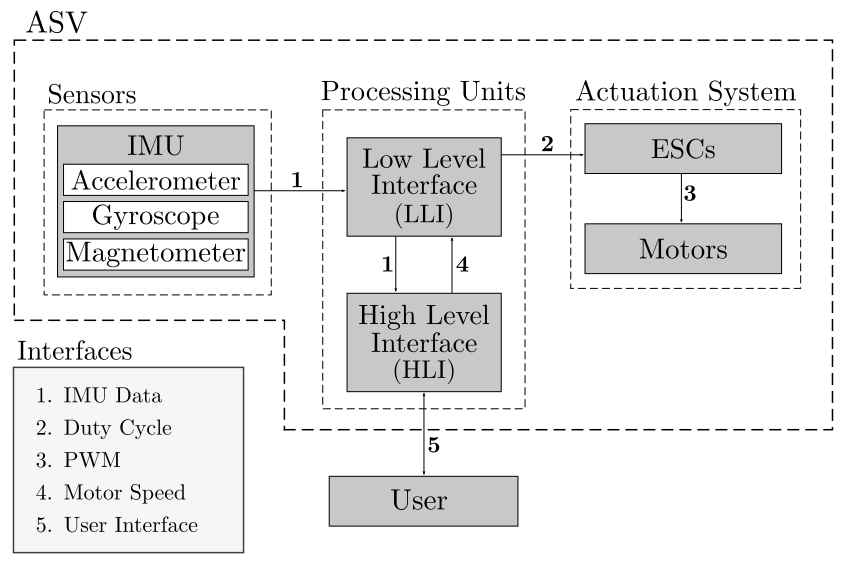
\includegraphics[width=.65\textwidth]{figures/systemDiagram4}
    \caption{Functional diagram of the given system.}
    \label{fig:systemDiagram}
\end{figure}
%
%The main parts of the system are the actuation system, the sensors and the processing units, see \autoref{fig:systemDiagram}. The processing unit gathers information from the IMU. This is handled by the Low Level Interface (LLI) which then sends it to the High Level Interface (HLI) where the control algorithms are implemented. The calculated actuation is then sent back to the LLI that sends the command to the actuation system. The ESCs (electronic speed controllers) then calculate the required signal to make the motors turn at the requested speed.

The main parts of the system are the actuation system, the sensors and the processing units, see \autoref{fig:systemDiagram}. The inertial measurement unit (IMU) information is gathered by the low level interface (LLI), and then transferred to the high level interface (HLI). In the HLI, the control algorithms are implemented, and the calculated commands are sent back to the actuation system through the LLI. The electronic speed controllers (ESCs) then calculate the required signal to make the motors turn at the requested speed.

This chapter briefly describes the main components of the surface vessel used in this project. Some additions to the existing systems are also presented.


    \section{Actuators}

Forward and side thrusters

motors

ESCs

how to obtain a force on the actuators
    \section{Sensors}\label{sec:sensors}
The control system designed in the vessel requires the presence of sensor data that provides information about the vessel's motion. This is handled by an IMU.

The IMU installed in the vessel is formed by a triaxial gyroscope with a digital range scaling between $\pm300^{\circ}$ s$^{-1}$, a triaxial accelerometer with a range of $\pm$18 g and a triaxial magnetometer with a range of $\pm$\num{2.5} G. It also contains a serial peripheral interface (SPI) to obtain the data. \cite{IMUDatasheet}
%
\begin{figure}[H]
	\includegraphics[width=0.2\textwidth]{figures/IMU}
	\caption{ADIS16405BMLZ IMU module mounted in the vessel \cite{IMUFigure}}
	\label{fig:IMU}
\end{figure}
%
The data provided by the IMU is used to estimate both the position and the attitude of the vessel.

%Triaxial, digital gyroscope with digital range scaling
%±75°/sec, ±150°/sec, ±300°/sec settings
%Tight orthogonal alignment, 0.05°
%Triaxial, digital accelerometer, ±18 g
%Triaxial, digital magnetometer, ±2.5 gauss
%SPI-compatible serial interface
%Embedded temperature sensor
%Single-supply operation: 4.75 V to 5.25 V

%\subsection{GPS}
%The vessel has a UP-501 GPS Receiver installed. It operates with a update frequency up to 10 Hz and its trasmits the received position data through a serial communication to the Low Level Interface. \cite{GPS}
%
%\begin{figure}[H]
%	\includegraphics[width=0.3\textwidth]{figures/GPS}
%	\caption{UP-501 GPS receiver mounted in the vessel \cite{GPS}.}
%	\label{fig:GPS}
%\end{figure}
%%
%As the UP-501 is a standard GPS receiver, its precision is in the range of meters \fxnote{How to prove this?? Maybe make a test.}. This makes it cumbersome to control the position of the vessel using only GPS data, and thus, the GPS and the IMU data is combined to obtained the position of the vessel.
    \section{Control System}\label{sec:ControlComputation}
\fxnote{Check the title os the section}

HLI - Computer( maybe wait until we know )

LLI - Arduino Interface to HLI bla bla


    
    %---------- Chapter 4 ---------------------------------------- Modeling
    \chapter{System Model} \label{chap:model}
The model of the surface vessel is based in the methods presented in \cite{TFossen}, where the principal effects that affect the behavior of the vessel are taken into account are described in order to generate a model that serves as a basis for control design and simulations.\fxnote{write pages in the source}



    \section{Reference Frames}\label{sec:frames}
The attitude and position of the vessel is described using two coordinate frames, a body frame and an inertial frame. For operations in a local area, with longitude and latitude approximately constants (flat navigation) a NED system (North-East-Down) can be assumed as an inertial frame where Newtonian mechanics apply \cite[p. 17]{TFossen}.

To distinguish between the two frames, the body frame is denoted with a subindex "$_\mathrm{b}$", and the inertial frame with subindex "$_\mathrm{n}$". In \autoref{fig:refFrame}, a diagram of the surface vessel with the notation used can be seen.
\begin{figure}[H]
    \includegraphics[width=0.6\textwidth]{figures/boat3D}
    \caption{$x_\mathrm{b}$, $y_\mathrm{b}$ and $z_\mathrm{b}$ refer to the position with respect to the body coordinate frame, while $x_\mathrm{n}$, $y_\mathrm{n}$ and $z_\mathrm{n}$ describe it with respect to the inertial frame. $\phi$, $\theta$ and $\psi$ refer to the rotation around $x_\mathrm{b}$, $y_\mathrm{b}$ and $z_\mathrm{b}$, respectively.}
    \label{fig:refFrame}
\end{figure}

The transformation from the body frame to the inertial can be done through a rotation matrix, \eqref{eq:RotMatrix}, which describes a total rotation in terms of three consecutive rotations. Note that due to the size of the matrices sine and cosine are denoted $s$ and $c$ respectively.

In this case the rotation matrix is composed with a 1-2-3 convention, that is, first a rotation around $x_{\mathrm{b}}$, then around $y_{\mathrm{b}}$ and finally around $z_{\mathrm{b}}$ \cite[p. 22]{TFossen}.

\begin{minipage}{0.32\linewidth}
    \begin{flalign}
    \vec{R}_\mathrm{X} &=
    \begin{bmatrix}
    1 & 0      & 0       \\ 
    0 & c\phi  & -s\phi  \\ 
    0 & s\phi  & c\phi   \nonumber  
    \end{bmatrix}\ , 	\label{eq:RotMatrix1}
    \end{flalign}
\end{minipage}\hfill
\begin{minipage}{0.32\linewidth}
    \begin{flalign}
    \vec{R}_\mathrm{Y} &=
    \begin{bmatrix}
    c\theta  & 0  & s\theta  \\ 
    0          & 1  & 0      \\ 
    -s\theta & 0  & c\theta  \nonumber 
    \end{bmatrix}\ , 	\label{eq:RotMatrix2}
    \end{flalign}
\end{minipage}\hfill
\begin{minipage}{0.32\linewidth}
    \begin{flalign}
    \vec{R}_\mathrm{Z} &=
    \begin{bmatrix}
    c\psi & -s\psi  & 0  \\ 
    s\psi & c\psi   & 0  \\ 
    0       & 0         & 1  \nonumber 
    \end{bmatrix}\ , 	\label{eq:RotMatrix3}
    \end{flalign}
\end{minipage}\hfill
{\small
\begin{flalign}
\vec{R}^\mathrm{n}_\mathrm{b} = \vec{R}_Z \vec{R}_Y \vec{R}_X =
\begin{bmatrix}
c\theta c\psi  & s\phi s\theta c\psi -c\phi s\psi  & c\phi s\theta c\psi + s\phi s\psi  \\ 
c\theta s\psi  & s\phi s\theta s\psi + c\phi c\psi & c\phi s\theta s\psi - s\phi c\psi  \\ 
-s\theta         & s\phi c\theta                           & c\phi c\theta
\end{bmatrix} \ .	\label{eq:RotMatrix}
\end{flalign}}

%
\begin{where}
    \va{\vec{R}_\mathrm{X}}{is the matrix describing a rotation around the $x_\mathrm{b}$ axis}{}
    \va{\vec{R}_\mathrm{Y}}{is the matrix describing a rotation around the $y_\mathrm{b}$ axis}{}
    \va{\vec{R}_\mathrm{Z}}{is the matrix describing a rotation around the $z_\mathrm{b}$ axis}{}
    \va{\vec{R}^\mathrm{n}_\mathrm{b}}{is the total rotation matrix}{}
\end{where}

To describe a vector in the inertial frame given its description in the body frame, it is left multiplied by the rotation matrix as
%
\begin{flalign}
v_{\mathrm{n}}=\vec{R}^\mathrm{n}_\mathrm{b}v_\mathrm{b}\ . 
\end{flalign}
\begin{where}
    \va{v_{\mathrm{n}}}{is a column vector that contains the description with respect to the inertial frame}{}
    \va{v_{\mathrm{b}}}{is a column vector that contains the description with respect to the body frame}{}
\end{where}

If the inverse computation is needed, it is done following the same procedure using $\vec{R}^\mathrm{n\ T}_\mathrm{b}$ as the rotation matrix.    

\subsection{Rigid Body Dynamics}

The first step to model the motion of the surface vessel is to look at its rigid body dynamics. They are described assuming that the center of gravity of the boat coincides with the origin of the body coordinate frame.

The translational movement can be analyzed using Newton's second law, where the acceleration of the vessel is related to the applied forces as
%
\begin{flalign}
\sum F=m \ddot{x} \ .
\end{flalign}

For rotational movements, the motion is described using the Newton's second law applied to rotational movement, where the torques applied to the system influence the angular acceleration around each axis as
%
\begin{flalign}
\sum \tau=I \ddot{\theta}\ .
\end{flalign}

%The movement can be influence by the Coriolis effect, due to the fact that the body coordinate frame rotates with respect to the inertial frame. This effect, however, can be neglected in the case of a small vehicle that moves slow such as the vessel at hand \finite{find source}.
The rotational movement is affected by the Coriolis effect, which appears if the vessel is not rotating around the axis with least or highest inertial axis. However, the influence of this force is small if the vessel rotates at low speeds, hence it has been neglected in the model.  \cite[p. 170]{TFossen}

\section{Hydrostatics}
The hydrostatics describe what forces and torques are applied on the surface vessel by the volume of fluid displaced when floating on water. The force induced upon the vessel is called buoyancy force and it is applied to the center of buoyancy.  

The buoyancy force acts in the negative $z_\mathrm{n}$ direction as seen in
%
\begin{flalign}
B = \rho g (V + \Delta V(z))\ .
\end{flalign}
%
\begin{where}
    \va{\rho}{is the density of the fluid in which the vessel floats}{kg \cdot  m^{-3}}
    \va{g}{is the gravitational acceleration}{m \cdot s^{-2}}
    \va{V}{is the volume of fluid displaced by the surface vessel}{m^3}
    \va{\Delta V}{is the change in volume of fluid displaced by the surface vessel}{m^3}
    \va{B}{is the buoyancy force}{N}
\end{where}

When the vessel floats, the gravity force cancels out $ \rho g V $ of the buoyancy force, making the contribution of the latest along $x_\mathrm{b}$, $y_\mathrm{b}$ and $z_\mathrm{b}$ directions dependent only on the variation with respect to the equilibrium flotation point.
This result is seen in 
%
\begin{flalign}
F_{z_\mathrm{n}} = mg - \rho g V -\rho g  \Delta V(z) = -\rho g  \Delta V(z) \ .
\end{flalign}
\begin{where}
    \va{F_{z_\mathrm{n}}}{is the summation of forces along the $z_\mathrm{n}$ direction}{N}
\end{where}

The change in volume can be expressed as in \autoref{eq:deltaV}. The water plane of the vessel is not considered to vary significantly with change in vertical position, thus the approximation seen in the following equation is applied
%
\begin{flalign}
\Delta V(z) = \int_{0}^{z_\mathrm{N}}A_\mathrm{wp}(\zeta)d\zeta \approx A_\mathrm{wp}z_\mathrm{n} \ .
\label{eq:deltaV}
\end{flalign}
\begin{where}
    \va{A_\mathrm{wp}}{is the water plane area of the vessel}{m^2}
\end{where}

The contribution along the body frame directions is calculated as a function of the $\phi$ and $\theta$ angles in  
%
\begin{flalign}
F_{x_\mathrm{b}} &= -\rho g A_\mathrm{wp}z_\mathrm{n} (-\sin \theta)  \ , \\
F_{y_\mathrm{b}} &= -\rho g A_\mathrm{wp}z_\mathrm{n} (\cos \theta \sin   \phi) \ , \\
F_{z_\mathrm{b}} &= -\rho g A_\mathrm{wp}z_\mathrm{n} (\cos \theta \cos  \phi) \ .
\label{eq:forcez}
\end{flalign}

%If the variations of $\phi$ and $\theta$ are small, the contribution of the buoyancy force in the $x_\mathrm{b}$ and $y_\mathrm{b}$ directions can be neglected and not included in the final model of the vessel. \cite[pp. 62-67]{TFossen}

The buoyancy force also contributes with some torques around the different axis in the body coordinate frame. This occurs as the center of buoyancy in general is not aligned with the center of gravity, generating some restoring torques on the vessel. These are dependent on the gravity and the buoyancy force. As the contribution of the term $\rho g \Delta V$ is small compared to that of $\rho g V$, only the latter is considered in the model \cite[pp. 62-67]{TFossen}. These torques are expressed as
%
\begin{flalign}
T_{\phi} &= -\rho g V \overline{GM}_{\mathrm{T}} \sin \phi (\cos \theta \cos \phi)   \ ,
\label{eq:torqphi} \\
T_{\theta} &= -\rho g V \overline{GM}_{\mathrm{L}} \sin \theta (\cos \theta \cos \phi) \ .
\label{eq:torqtheta}
\end{flalign}
\begin{where}
    \va{T_{\phi}}{is the restoring torque due to the buoyancy force in the $\phi$ direction}{N \cdot m}
    \va{T_{\theta}}{is the restoring torque due to the buoyancy force in the $\theta$ direction}{N \cdot m}
    \va{\overline{GM}_\mathrm{T}}{is the transverse metacentric height}{m}
    \va{\overline{GM}_\mathrm{L}}{is the longitudinal metacentric height}{m}
\end{where}

The metacentric heights are the distances between the center of gravity and the metacenter of the vessel. The metacenter position the intersection of imaginary vertical lines that go through the different centers of buoyancy originated when tilting or displacing the vessel. This height can be seen in \autoref{fig:app_metacentric}.

\begin{figure}[H]
    %\includegraphics[width=0.5\textwidth]{figures/app_metacentric}
    \caption{\cite[p. 62]{TFossen} \fxnote{include figure from book}}
    \label{fig:app_metacentric}
\end{figure}

\section{Hydrodynamics}
The hydrodynamic forces induced in the surface vessel are mainly caused by two terms. The added mass and the viscous damping.

The added mass induces a force that originate from the vessel imposing some energy in the surrounding fluid when the vessel moves through it, which is dependent on the acceleration of the vessel. However, this effect is neglected since most of the effective mass of the vessel comes from the nominal mass, and any variation is handled by the controller.

The viscous damping is a combination of several factors, namely, skin friction, wave drift damping and vortex shedding \cite[p. 122]{TFossen}. This type of damping appears in the equations as coefficients that multiply, with negative sign, the different translational and angular velocities that define the movement of the vessel. For each degree of freedom it is expressed as
%
\begin{flalign}
D_{\dot{x}_\mathrm{b}} &= - d_{\dot{x}_\mathrm{b}}  \dot{x}_\mathrm{b}\ , \\
D_{\dot{y}_\mathrm{b}} &= - d_{\dot{y}_\mathrm{b}}  \dot{y}_\mathrm{b}\ , \\
D_{\dot{z}_\mathrm{b}} &= - d_{\dot{z}_\mathrm{b}}  \dot{z}_\mathrm{b}\ , \\
D_{\dot{\phi}} &= - d_{\dot{\phi}}                  \dot{\phi}\ , \\
D_{\dot{\theta}} &= - d_{\dot{\theta}}              \dot{\theta}\ , \\
D_{\dot{\psi}} &= - d_{\dot{\psi}}                  \dot{\psi}\ .  \\
\end{flalign}
\begin{where}
    \va{D_{i}}{is the damping force or torque due to viscous damping}{N, \ N \cdot m}
    \va{d_{i}}{is the viscous damping coefficient}{N \cdot m^{-1} \cdot s, \ N \cdot m \cdot rad^{-1} \cdot s}
\end{where}

These equations consider that the viscous friction is linear, since this assumption can be done for vessel speeds lower than 2 m/s \cite[p. 138]{TFossen}. 

    \section{Model Equations}   
The final model equations are presented in this section.
The model equations will be presented, linarized and put into state space.
\autoref{fig:boat3DForces} and \ref{fig:boat2D} show a diagram of the vessel.
The model equations are presented in to body frame, meaning all movement is relative to the boat. 
The states can be transformed into the inertial frame, using equation \autoref{eq:RotMatrix}.  
\begin{figure}[H]
    \captionbox  %<--use captionbox instead if no global caption is needed
    {               %                                \%-%-%-%-%-%-%\
        Diagram of the boat where the forces applied by the motors are shown.                %\
        \label{fig:boat3DForces}                                  %\
    }                                                                 %\
    {                                                                  %\
        \includegraphics[width=.46\textwidth]{figures/boat3DForces}         %\
    }                                                                    %\
    \hspace{5pt}                                                          %\
    \captionbox  %<-----------------------------------------------------%\
    {       
        Above perspective of the vessel, where the distances needed for the model equations are presented.                                                                %\                         %\
        \label{fig:boat2D}                                     %\
    }                                                                           %\
    {                                                                            %\
        \includegraphics[width=.2\textwidth]{boat2D}            %|
    }                                                                             %|
\end{figure}
%
The translational movement of the vessel is described by \autoref{eq:x_pos_model}, \ref{eq:y_pos_model} and \ref{eq:z_pos_model}.
The model relates the forces applied by the motors to the boat frame. 
%
\begin{flalign}
	m_\mathrm{x} \ddot{x}_\mathrm{b} &=  F_\mathrm{1} + F_\mathrm{2}  - d_{\dot{x}_\mathrm{b}} \dot{x}_\mathrm{b} + F_{x_\mathrm{b}}
    \label{eq:x_pos_model} \\
    m_\mathrm{y} \ddot{y}_\mathrm{b} &=  -d_{\dot{y}_\mathrm{b}} \dot{y_\mathrm{b}} + F_{y_\mathrm{b}}
    \label{eq:y_pos_model} \\
    m_\mathrm{z} \ddot{z}_\mathrm{b} &=  -d_{\dot{z}_\mathrm{b}}\dot{z_\mathrm{b}} + F_{z_\mathrm{b}} \label{eq:z_pos_model}
\end{flalign}
%
\begin{where}
	\va{m_\mathrm{x,y,z}}{Is the virtual mass in their respective direction}{kg}
%    \va{m_\mathrm{x}}{}{kg}
%    \va{m_\mathrm{y}}{}{kg}
%    \va{m_\mathrm{z}}{}{kg}
    \va{\ddot{x}_\mathrm{b}}{is the acceleration in the $x_\mathrm{b}$ direction}{m s^{-2}}
    \va{\ddot{y}_\mathrm{b}}{is the acceleration in the $y_\mathrm{b}$ direction}{m s^{-2}}
    \va{\ddot{z}_\mathrm{b}}{is the acceleration in the $z_\mathrm{b}$ direction}{m s^{-2}}
    \va{\dot{x}_\mathrm{b}}{is the velocity in the $x_\mathrm{b}$ direction}{m s^{-1}}
    \va{\dot{y}_\mathrm{b}}{is the velocity in the $y_\mathrm{b}$ direction}{m s^{-1}}
    \va{\dot{z}_\mathrm{b}}{is the velocity in the $z_\mathrm{b}$ direction}{m s^{-1}}
    \va{F_1}{is the force applied by motor 1}{N}
    \va{F_2}{is the force applied by motor 2}{N}
\end{where} \\
% 
From the equations it shows that only the x-axis on the boat frame is controllable, as this is the axis containing the main thrusters. 
While the vessel do contain side thrusters, they are only intended for fine maneuvering, as their strength is relatively weak, compared to the main thrusters.\\
%
The virtual mass components is the added mass from the displaced water in the respective direction plus the mass of the vessel.
This value will be different for each axis, as the difference in shape drags a different amount of water with it depending on the direction.
    
The angular movement of the vessel is described by \autoref{eq:phi_model}, \ref{eq:theta_model} and \ref{eq:psi_model}.

\begin{flalign}
    I_\mathrm{x}\ddot{\phi} &= -d_{\dot{\phi}} \dot{\phi} + T_\mathrm{\phi}  
    \label{eq:phi_model} \\
    I_\mathrm{y}\ddot{\theta} &= -d_{\dot{\theta}} \dot{\theta} + T_\mathrm{\theta}  
    \label{eq:theta_model} \\
    I_\mathrm{z}\ddot{\psi} &= F_\mathrm{1}l_\mathrm{1} - F_\mathrm{2} l_\mathrm{2} - d_{\dot{\psi}} \dot{\psi} \label{eq:psi_model}
\end{flalign}
%
\begin{where}
    \va{I_\mathrm{x}}{is the inertia around the $x_\mathrm{b}$ axis}{kg}
    \va{I_\mathrm{y}}{is the inertia around the $y_\mathrm{b}$ axis}{kg}
    \va{I_\mathrm{z}}{is the inertia around the $z_\mathrm{b}$ axis}{kg}
    \va{\ddot{\phi}}{is the angular acceleration around the $x_\mathrm{b}$ axis}{rad s^{-2}}
    \va{\ddot{\theta}}{is the angular acceleration around the $y_\mathrm{b}$ axis}{rad s^{-2}}
    \va{\ddot{\psi}}{is the angular acceleration around the $z_\mathrm{b}$ axis}{rad s^{-2}}
    \va{\dot{\phi}}{is the angular velocity around the $x_\mathrm{b}$ axis}{rad s^{-1}}
    \va{\dot{\theta}}{is the angular velocity around the $y_\mathrm{b}$ axis}{rad s^{-1}}
    \va{\dot{\psi}}{is the angular velocity around the $z_\mathrm{b}$ axis}{rad s^{-1}}
    \va{l_1}{is the perpendicular distance from motor 1 to the center of gravity}{m}
    \va{l_2}{is the perpendicular distance from motor 2 to the center of gravity}{m}
\end{where}

Similar to the translatoric equations, only one axis is controllable, due to the lack of actuators. 
This will not be a problem in practice, as yaw is the only direction that it desirable to control, and any torque induced upon the other axis is a be product of the dynamics.

    \section{Linearization of Model Equations}\label{sec:linearizationModel}
The model equations need to be linearized to be able to design a controller using linear techniques. This is done using the first order Taylor approximation around an equilibrium as seen in 
\begin{flalign}
    f(x) &\approx f(\overline{x}) + f'(\overline{x}) (x-\overline{x})  \rightarrow\ \tilde{f}(x) \approx f'(\overline{x}) \tilde{x}
    \label{taylor}
\end{flalign}
In this equation, $\overline{x}$ represents the equilibrium point and $\tilde{x}$ the equilibrium point.

The equilibrium point must fulfill that all the derivatives of the states are zero, in this case the velocities and accelerations. This also result in the restoring forces and torques, as well as the motor forces equal to zero. 

To apply the approximation, the function must be differentiated with respect to each of the present variables, and once linearized, the function is expressed in terms of variations from the equilibrium point.
%
\begin{flalign}
    f &= f(x_1,x_2,...,x_\mathrm{n}) \nonumber \\
    \tilde{f}&=\frac{\partial f}{\partial x_1}\bigg|_{\overline{x}_1,\overline{x}_2,...,\overline{x}_n}\ \tilde{x}_1 + \frac{\partial f}{\partial x_2}\bigg|_{\overline{x}_1,\overline{x}_2,...,\overline{x}_n}\ 
    \tilde{x}_2+...+ \frac{\partial f}{\partial x_n}\bigg|_{\overline{x}_1,\overline{x}_2,...,\overline{x_n}}\ \tilde{x}_\mathrm{n} \nonumber
    \label{eq:dummytaylor}
\end{flalign}

In the case of the boat, the only non-linear terms are the restoring forces and torques. They can be linearized and give the result seen in 
%
\begin{flalign}
    \tilde{F}_{x_\mathrm{b}} &= 0  \label{eq:forcexlin}\\
    \tilde{F}_{y_\mathrm{b}} &= 0  \label{eq:forceylin}\\
    \tilde{F}_{z_\mathrm{b}} &= -\rho g A_\mathrm{wp} \tilde{z}_\mathrm{n} \label{eq:forcezlin} \\
 	\tilde{T}_{\phi} &= -\rho g V \overline{GM_{L}}\cdot \tilde{\phi} \label{eq:torquephilinar} \\
    \tilde{T}_{\theta} &= -\rho g V \overline{GM_{L}}\cdot \tilde{\theta}\label{eq:torquethetalinar}   
\end{flalign}

The first order Taylor approximation is only applicable in areas close to the operating point, however as the vessel should not deviate much from this during operation. 

From now on, the linearized variables are represented without the symbol $\Delta$, to avoid excessive notation, even though they refer to changes with respect to the the equilibrium point.

The model equations including these linearized terms end up being
%
\begin{flalign}
 	m_\mathrm{x} \ddot{x}_\mathrm{b} &=  F_\mathrm{1} + F_\mathrm{2}  - d_{\dot{x}_\mathrm{b}} \dot{x}_\mathrm{b}
     \label{eq:x_pos_model_lin} \\
    m_\mathrm{y} \ddot{y}_\mathrm{b} &=  -d_{\dot{y}_\mathrm{b}} \dot{y_\mathrm{b}}
     \label{eq:y_pos_model_lin} \\
    m_\mathrm{z} \ddot{z}_\mathrm{b} &=  -d_{\dot{z}_\mathrm{b}}\dot{z_\mathrm{b}} -\rho g A_\mathrm{wp} \tilde{z}_\mathrm{n} \label{eq:z_pos_model_lin}   \\
    I_\mathrm{x}\ddot{\phi} &= -d_{\dot{\phi}} \dot{\phi} - \rho g V \overline{GM_{L}}\cdot \tilde{\phi} 
    \label{eq:phi_model_limn} \\
    I_\mathrm{y}\ddot{\theta} &= -d_{\dot{\theta}} \dot{\theta} - \rho g V \overline{GM_{L}}\cdot \tilde{\theta} 
    \label{eq:theta_model_lin} \\
    I_\mathrm{z}\ddot{\psi} &= F_\mathrm{1}l_\mathrm{1} - F_\mathrm{2} l_\mathrm{2} - d_{\dot{\psi}} \dot{\psi} \label{eq:psi_model_lin}
\end{flalign}



%\begin{flalign}
%    m_\mathrm{x} \ddot{x}_\mathrm{b} &=  F_\mathrm{1} + F_\mathrm{2}  - d_\mathrm{x} \dot{x}_\mathrm{b} + m_\mathrm{y} \dot{y_\mathrm{b}} \dot{\psi} - m_\mathrm{z} \dot{z}_\mathrm{b} \dot{\theta} - F_\mathrm{x}
%    \label{eq:x_pos_model} \\
%    m_\mathrm{y} \ddot{y_\mathrm{b}} &=  -d_\mathrm{y}\dot{y_\mathrm{b}}-m_\mathrm{x}\dot{x_\mathrm{b}}\dot{\psi}+m_\mathrm{z}\dot{z_\mathrm{b}}\dot{\phi}-F_\mathrm{y}
%    \label{eq:y_pos_model} \\
%    m_\mathrm{z} \ddot{z_\mathrm{b}} &=  -d_\mathrm{z}\dot{z_\mathrm{b}}+ m_\mathrm{b}\dot{x_\mathrm{b}}\dot{\theta}-m_\mathrm{y}\dot{y_\mathrm{b}} \dot{\phi}-F_\mathrm{z} \label{eq:z_pos_model}
%\end{flalign}
%
%\begin{flalign}
%    I_\mathrm{x}\ddot{\phi} &= -d_\mathrm{\phi} \dot{\phi}-(m_\mathrm{z}-m_\mathrm{y}) \dot{z}_\mathrm{b} \dot{y}_\mathrm{b}-(I_\mathrm{z}-I_\mathrm{y}) \dot{\theta } \dot{\psi}+T_\mathrm{\phi}  
%    \label{eq:x_inert_model} \\
%    I_\mathrm{y}\ddot{\theta} &= -d_\mathrm{\theta} \dot{\theta}-(m_\mathrm{z}-m_\mathrm{x}) \dot{x}_\mathrm{b} \dot{y}_\mathrm{b}-(I_\mathrm{x}-I_\mathrm{z}) \dot{\phi} \dot{\psi}+T_\mathrm{\theta}  
%    \label{eq:y_inert_model} \\
%    I_\mathrm{z}\ddot{\psi} &= -d_\mathrm{\psi} \dot{\psi}-(m_\mathrm{y}-m_\mathrm{x}) \dot{x}_\mathrm{b}\dot{y}_\mathrm{b}-(I_\mathrm{z}-I_\mathrm{y})\dot{\psi}\dot{\theta}+F_\mathrm{1}l_\mathrm{1}+F_\mathrm{2}l_\mathrm{2}+T_\mathrm{\psi} \label{eq:z_inert_model}
%\end{flalign}

    
    %---------- Chapter 5 ---------------------------------------- Controller Design
    \chapter{Inner Controller Design}

Header of control chapter

\begin{figure}[H]
    \includegraphics[width=0.8\textwidth]{figures/controllerDiagram}
    \caption{}
    \label{fig:controllerDiagram}
\end{figure}
    \section{State Space Model}\label{chap:control}

The linearized model derived in \autoref{sec:linearizationModel}, consisting of \autoref{eq:x_pos_model_lin} to \ref{eq:psi_model_lin}, needs to be represented in state space form in order to design a state space controller. In order to do that, the 3 degree of freedom model used for the control of the vessel is represented as
\begin{flalign}
  \vec{\dot{x}}(t) &= \vec{A} \vec{x}(t) + \vec{B} \vec{u}(t)
  \label{xDotLinear} \\
  \vec{y}(t) &= \vec{C} \vec{x}(t) + \vec{D} \vec{u}(t)
  \label{yLinear} 
\end{flalign}
\begin{where}
  \va{\vec{x}}{is the state vector}{}
  \va{\vec{u}}{is the input vector}{}
  \va{\vec{y}}{is the output vector}{}
  \va{\vec{A}}{is the state matrix}{}
  \va{\vec{B}}{is the input matrix}{}
  \va{\vec{C}}{is the output matrix}{}
  \va{\vec{D}}{is the feed-forward matrix}{}
\end{where}
%
The state vector is constituted by the angle and velocity in yaw as well as the velocity in x in the body frame. The outputs of the system are yaw angle and velocity in x in the body frame. The input to the system is composed of the two forces applied in the body frame.
%It is important to notice that the position of the vessel in the body reference frame represents the  integration of the velocity along the body frame directions.
%This can also be seen as the position of the vessel with respect to a frame whose origin coincides with that of the NED frame and whose orientation coincides with that of the body frame \cite[p. 173]{TFossen}. 

\begin{minipage}{0.32\linewidth}
  \begin{flalign}
    \vec{x(t)} = 
    \begin{bmatrix}
      \psi\\
      \dot{\psi}\\
      \dot{x}_{b} \\
    \end{bmatrix} \nonumber
    \label{xVector}
  \end{flalign}  
\end{minipage}\hfill
%\hspace{0.03\linewidth}
\begin{minipage}{0.32\linewidth}
  \begin{flalign}
    \vec{y(t)} = 
    \begin{bmatrix}
      \phi \\
      \dot{x}_{b} \\
    \end{bmatrix} \nonumber
    \label{yVector}
  \end{flalign}
\end{minipage}\hfill
%\hspace{0.03\linewidth}
\begin{minipage}{0.32\linewidth}
  \begin{flalign}
    \vec{u(t)}= 
    \begin{bmatrix}
      F_1 \\
      F_2 
    \end{bmatrix}
    \label{uVector}
  \end{flalign} \nonumber
\end{minipage}\hfill

The resulting $\vec{A}$, $\vec{B}$, $\vec{C}$ and $\vec{D}$ matrices are
\begin{flalign}
  \vec{A} &=
  \begin{bmatrix}
    \ 0 & 1                   & 0                \ \ \ \\ 
    \ 0 & -\frac{d_\psi}{I_z} & 0                \ \ \ \\ 
    \ 0 & 0                   & -\frac{d_x}{m_x} \ \ \     
  \end{bmatrix}\rule{30px}{0px}
    \vec{B} = 
  \begin{bmatrix}
    \ 0               & 0                \ \ \ \\
    \ \frac{l_1}{I_z} & -\frac{l_2}{I_z} \ \ \ \\   
    \ \frac{1}{m_x}   & \frac{1}{m_x}    \ \ \
  \end{bmatrix}\rule{30px}{0px}
  \vec{C} =   
  \begin{bmatrix}
    \ 1 & 0 & 0  \ \ \ \\ 
    \ 0 & 0 & 1  \ \ \    
  \end{bmatrix}
   \label{eqStateSpaceABC}
\end{flalign}
and the $\vec{D}$ matrix is zero.

    \section{Initial Control Design}
%
It is desired to design a state feedback using a linear quadratic regulator (LQR). As the controller eventually must be implemented the design is carried out in the discrete domain. To do so, it is necessary to discretize the system. A discrete state space model can be expressed as,
%
\begin{flalign}
  \vec{x}(k+1) &= \vec{A_z} \vec{x}(k) + \vec{B_z} \vec{u}(k)
  \label{xDotLinearDiscrete} \\
  \vec{y}(k)   &= \vec{C_z} \vec{x}(k) + \vec{D_z} \vec{u}(k) \ \ ,
  \label{yLinearDiscrete} 
\end{flalign}
%
where the z subindexes indicate the matrices being in the discrete domain and k is the sample index. The model is discretized using zero order hold. In \autoref{fig:discreteSSBlock} the discrete system is shown in a block diagram. The feed forward matrix is excluded as it is not present in this system.
%
\begin{figure}[H]
  \includegraphics[width=0.6\textwidth]{figures/discreteSystemBlockDiagram}
  \caption{Block diagram of the discrete system without feed forward.}
  \label{fig:discreteSSBlock}
\end{figure}
%
\fxnote{talk about controllability here.}
%
In order to track a reference and handle input disturbances, it is chosen to also include an integral controller in the design. The final control structure is seen in \autoref{fig:blockConrolDesignLQR}.
%
\begin{figure}[H]
  \includegraphics[width=0.9\textwidth]{figures/integralControlBlockDiagram}
  \caption{Block diagram of the control structure in the discrete domain.}
  \label{fig:blockConrolDesignLQR}
\end{figure}
%
To design this feedback system, it is convenient to express it on the following form:
\begin{flalign}
  \vec{x_e}(k+1) &= \vec{A_e} \vec{x}(k) + \vec{B_e} \vec{u}(k) + \vec{r}(k)
  \label{eq:xDotLinearDiscrete} \\
  \vec{y}(k)     &= \vec{C_e} \vec{x}(k)  \ \ .
  \label{eq:yLinearDiscrete} 
\end{flalign}
%
To describe the control design in this form, the $\vec{A_e}$, $\vec{B_e}$ and $\vec{C_e}$ matrices must be constructed. From \autoref{fig:blockConrolDesignLQR}, following relation is found:
%
\begin{flalign}
  \vec{x_I}(k+1) &= \vec{x_I}(k) + \vec{y}(k) + \vec{r}(k)    \nonumber \\
  \vec{x_I}(k+1) &= \vec{x_I}(k) - C_z \vec{x}(k) + \vec{r}(k)  \ \ .
  \label{eq:xIDiscrete}
\end{flalign}
%
This leads to the discrete state space model extended with the integral state expressed as
%
\begin{flalign}
  \begin{bmatrix}
    \vec{x}(k+1)  \\
    \vec{x_I}(k+1)
  \end{bmatrix}
  =
  \begin{bmatrix}
    \vec{A}_{\vec{z}_{3x3}} & \vec{O}_{_{3x2}} \\
   -\vec{C}_{\vec{z}_{2x3}} & \vec{I}_{_{2x2}} \\
  \end{bmatrix}
  \begin{bmatrix}
    \vec{x}(k)    \\
    \vec{x_I}(k)
  \end{bmatrix}
  +
  \begin{bmatrix}
    \vec{B}_{\vec{z}_{3x2}} \\
    \vec{O}_{2x2}
  \end{bmatrix}
  \vec{u}(k)
  +
  \begin{bmatrix}
    \vec{O}_{3x2} \\
    \vec{I}_{2x2}
  \end{bmatrix}
  \vec{r}(k)
  \label{eq:discreteSSWithIntegralX}
\end{flalign}  
%
\begin{flalign}
  \vec{y}(k)
  =
  \begin{bmatrix}
    \vec{C}_{\vec{z}_{2x3}} &  \vec{O}_{2x2}
  \end{bmatrix}
  \begin{bmatrix}
    \vec{x}(k)    \\
    \vec{x_I}(k)
  \end{bmatrix}  \ \ ,
  \label{eq:discreteSSWithIntegralY}
\end{flalign}  
%
which cooresponds to \autoref{eq:xDotLinearDiscrete} and \ref{eq:yLinearDiscrete}.

A discrete time infinite horizon LQR is used in the design of the feedback, $\vec{F_e} = [\ \vec{F} \ \ \vec{F}_\mathrm{I} ]\ $, which works by minimizing the cost function,
%
\begin{flalign}
  J = \sum_{k=0}^\infty \vec{x}_k^\mathrm{T}\vec{Q}\vec{x}_k + \vec{u}_k^\mathrm{T}\vec{R}\vec{u}_k \ dt \ \ .
\end{flalign}
\begin{where}
	\va{\vec{Q}}{is the state cost matrix}{}
  \va{\vec{R}}{is the input cost matrix}{}
\end{where}

The Q matrix contains the penalties for the state, such that a higher cost is generated for more critical states, thus driving these states faster to zero. The R matrix contains the penalties for the input. This helps to ensure that the actuators never enters saturation.
Bryson's rule is used to determine sensible values for the state and input penalties in the Q and R matrices.
%
\begin{flalign} 
Q_{ii} &= \frac{1}{[x_{i_\mathrm{max}}]^2} \ \ \ \ R_{ii} = \frac{1}{[u_{i_\mathrm{max}}]^2}
\label{eq:QRBryson}
\end{flalign}
\begin{where}
  \va{x_{i_\mathrm{max}}}{are the maximum acceptable state values}{}
  \va{u_{i_\mathrm{max}}}{are the maximum acceptable input values}{}
\end{where}

From this the state feedback is calculated by,
%
\begin{flalign} 
  \vec{F}_\mathrm{e} &= (\vec{R} \vec{B}_\mathrm{e}^\mathrm{T} \vec{P}\vec{B}_\mathrm{e})^{-1}  \vec{B}_\mathrm{e}^\mathrm{T} \vec{P}\vec{B}_\mathrm{e}
  \label{eq:QRFeedback}
\end{flalign}
\begin{where}
  \va{\vec{P}}{is the state transfer matrix.}{}
\end{where}

$\vec{P}$ provides a feedback matrix which minimizes the cost function, and can be found by use of the Riccatti equation.
%$\vec{F}_\mathrm{e}$ can be seperated to make F and F_I as the first 6 columns are state feedback and the last three are the integral control. These feedback matricees can can be implemented as shown in \autoref{fig:blockConrolDesignLQR}.












     	
    %---------- Chapter 6 ---------------------------------------- Path Following
    \chapter{Outer Controller Design}\label{chap:outerController}
fThe vessel functionality, as stated in \autoref{sec:requirements}, requires it to follow a path along which the bathymetric measurements are taken. The path is generated from the given area in straight lines as described in \autoref{sec:pathgeneration}.  The generated path is followed by using an enclosure based steering algorithm \cite[pp. 258-265]{TFossen} that uses waypoints sampled along the path. The outputs for this controller are the reference for the yaw angle and the velocity along the $x_\mathrm{b}$ axis, which are inputs to the state space controller designed in \autoref{chap:innercontrol}.
    \section{Path Following Algorithm}\label{sec:pathfollower}
The path generated is approximated by straight line segments connected by the calculated waypoints. The vessel then follows these in order to track the path and cover the area in which the measurements are to be taken. This approximation is suitable as the bathymetric measurements are usually taken in straight line paths. Straight line segments on the curved paths are not required as the curved paths are outside of the area of interest. If curved paths were required, the solution would be to sample the path with higher frequency in curved sections. \autoref{fig:pathandwaypoints} shows an example of how a path is approximated by straight line segments and waypoints.
\begin{figure}[H]
	\includegraphics[width=0.6\textwidth]{figures/pathandwpts}
	\caption{A predefined path and its approximation as straight line segments using waypoints.}
	\label{fig:pathandwaypoints}
\end{figure}
The algorithm starts by considering the first two waypoints in the path. The yaw reference given to the state space controller is calculated based on the crossing point between the straight line segment that joints the waypoints and a circle centered in the position of the boat. \autoref{fig:LOSalgorithm} shows how this crossing point is obtained. The crossing point is also called LOS (Line Of Sight) point and is found using the equations of the circle and of the straight line as
%
\begin{flalign}
	(&x_\mathrm{los}-x_\mathrm{n})^2 + (y_\mathrm{los}-y_\mathrm{n})^2 = R^2, \label{eq:circle} \ \\
	&y_\mathrm{los}-y_\mathrm{k} = \frac{y_\mathrm{k+1}-y_\mathrm{k}}{x_\mathrm{k+1}-x_\mathrm{k}}(x_\mathrm{los}-x_\mathrm{k}) \label{eq:line} 
\end{flalign}
\begin{where}
	\va{R}{is the radius of the circle centered at the vessel position}{}
	\va{[x_\mathrm{los},y_\mathrm{los}]}{is the crossing point between the circle around the vessel and the straight line that joins the waypoints}{}
	\va{[x_\mathrm{k},y_\mathrm{k}]}{is the first waypoint in the currently followed path segment}{}
	\va{[x_\mathrm{k+1},y_\mathrm{k+1}]}{is the second waypoint in the currently followed path segment}{}
	\va{[x_\mathrm{n},y_\mathrm{n}]}{is the position of the vessel in the NED frame}{}
\end{where}
%
\begin{figure}[H]
	\includegraphics[width=0.5\textwidth]{figures/LOSalgorithm}
	\caption{Algorithm used to find the yaw reference for the state space controller in order to follow a path.}
	\label{fig:LOSalgorithm}
\end{figure}
The LOS point is then used to calculate $\chi$ as the angle from the $x_\mathrm{n}$ axis and the line joining the position of the vessel and the LOS point. See \eqref{eq:chi}. This can be directly used as the reference for yaw, $\psi_\mathrm{ref}$, in the state space controller. This disregards the possibility of disturbances and assumes that the velocity vector of the vessel is aligned with the $x_\mathrm{b}$ axis. This is in general not true as disturbances like wind or waves would generate some speed also in the $y_\mathrm{b}$ axis direction. The reference for yaw is then adjusted by subtracting the angle that the velocity vector has with respect to the $x_\mathrm{b}$ axis as seen in \eqref{eq:beta} and \eqref{eq:psiref}. 

This approach tries to make the vessel velocity vector point towards the LOS point.
%
\begin{flalign}
	\chi &= \arctan\left(\frac{y_\mathrm{los}-y_\mathrm{n}}{x_\mathrm{los}-x_\mathrm{n}}\right), \label{eq:chi} \ \\
	\beta &= \arctan\left(\frac{\dot{y}_\mathrm{b}}{\dot{x}_\mathrm{b}}\right) \label{eq:beta}, \ \\
	\psi&_\mathrm{ref} = \chi - \beta. \label{eq:psiref}
\end{flalign}
\begin{where}
	\va{\chi}{is the angle between the $x_\mathrm{n}$ axis and the LOS point}{}
	\va{\beta}{is the angle between the velocity vector of the vessel and the $x_\mathrm{b}$ axis}{}
\end{where}
%
The algorithm relies on the path and the circle defined around the boat to cross at the LOS point. 

If the vessel is positioned far from the path such that the circle does not intersect it, then the algorithm uses the next waypoint as LOS point. Once the vessel gets closer to the path, the LOS point is calculated as described above.

The yaw reference, $\psi_\mathrm{ref}$, given to the controller in \ref{innercontrol} ensures that the vessel will follow the desired LOS.

In order to follow all the path, a way to change which two waypoints define the current path segment needs to be established. Several possibilities can be considered but all of them change active waypoints when the vessel gets close enough to the waypoint that defines the end of the segment. In the project at hand, the distance to the waypoint is evaluated as the distance from the waypoint to the intersection point of the path segment and a perpendicular line to the segment that passes through the vessel position. This distance is depicted in \autoref{fig:changewaypoints}.
\begin{figure}[H]
	\includegraphics[width=0.6\textwidth]{figures/LOSalgorithmdistancewp}
	\caption{The distance considered when defining the criterion to change to new waypoints.}
	\label{fig:changewaypoints}
\end{figure}
With this approach, the vessel will always try to move forward in the path although a waypoint position has not been precisely attained. % This avoids situations like the one shown in \autoref{fig:goingbackapproach} where the vessel turns around in order to hit the waypoint precisely.
This could be caused by a sudden disturbance experienced by the vessel and, in general, it is desired to keep following the path rather than turning around to hit the waypoint. In most cases, the vessel itself is going to be close to the waypoint when the change occurs. This can be seen in the simulation plots presented below. 

\subsection{Path Following Algorithm Simulation}

\fxnote{Do not include many graphs now because we will probably redo them. Just some dummy ones.} 
\fxnote{Maybe we could include the result also with different low level controllers}
The path following algorithm has been tested in the same path and considering different settings for the algorithm. In all cases, the radius of the circle defined around the vessel is 5 m and the distance in which the active waypoints are changed is 3 m. 

In \autoref{fig:simpleLOSalgorithm} and \ref{fig:simpleLOSalgorithmdisturbance} the results of the algorithm are presented when considering the simpler case in which $\psi_\mathrm{ref} = \chi$, that is, assuming the velocity of the vessel is pointing along the $x_\mathrm{b}$ direction. In the first graph the path is followed precisely as the assumption regarding the velocity vector holds,  whereas in the second, the constant disturbance imposes an offset in the position of the vessel.
\begin{figure}[H]
	\captionbox  %<--use captionbox instead if no global caption is needed
	{               %                                \%-%-%-%-%-%-%\
	 	Performance of the path following algorithm based on $\psi_\mathrm{ref}=\chi$.                %\
		\label{fig:simpleLOSalgorithm}                                  %\
	}                                                                 %\
	{                                                                  %\
		\includegraphics[width=.45\textwidth]{figures/pathfollowingsimple}         %\
	}                                                                    %\
	\hspace{5pt}                                                          %\
	\captionbox  %<-----------------------------------------------------%\
	{       
		Performance of the path following algorithm based on $\psi_\mathrm{ref}=\chi$. The vessel is experiencing a constant disturbance force of 1 N applied with an angle of $\pi/2$.                                                                  %\                         %\
		\label{fig:simpleLOSalgorithmdisturbance}                                     %\
	}                                                                           %\
	{                                                                            %\
		\includegraphics[width=.45\textwidth]{figures/pathfollowingsimpledist}            %|
	}                                                                             %|
\end{figure}
When the information of the vessel velocity is used to calculate the reference angle, $\psi_\mathrm{ref}$, the disturbance is rejected. This is seen in \autoref{fig:normalLOSalgorithmdisturbance}, where the vessel is experiencing the same disturbance as in \autoref{fig:simpleLOSalgorithmdisturbance}. In this case, the offset in position has been corrected and the path is precisely followed.
\begin{figure}[H]
	\includegraphics[width=0.5\textwidth]{figures/pathfollowingcomplex}
	\caption{Performance of the path following algorithm based on $\psi_\mathrm{ref}=\chi-\beta$. The vessel is experiencing a constant disturbance force of 1 N applied with an angle of $\pi/2$.}
	\label{fig:normalLOSalgorithmdisturbance}
\end{figure}
According to the results of the simulations, it can be said that the vessel hits the waypoints precisely when they are part of a straight line section of the path. In curved sections, the vessel joins smoothly the straight line segments that approximate the curve. In many cases, and especially for bathymetric measurements the algorithm can be considered suitable.

	




    
    %---------- Chapter 7 ---------------------------------------- Sensor Fusion
    \chapter{Sensor Fusion}\label{chap:sensorFusion}



    \section{Attitude Estimation}\label{sec:attFusion}
The attitude estimation is done using a Kalman filter. The estimate contains attitude, angular velocity and angular acceleration information. For constructing the Kalman filter, a process model and a measurement model need to be created. 

The process model describes the dynamics of the system and how the inputs affect its states. The process model includes also noise, which is assumed to be normally distributed.
The measurement model describes how the measurements taken from the IMU relate with the states of the system represented in the process model. Measurement noise is also included in the model. The process and measurement models are 
%
\begin{flalign}
    \vec{x}_\mathrm{att}(k+1) &= \vec{A}_\mathrm{att}\vec{x}_\mathrm{att}(k) + \vec{B}_\mathrm{att} \vec{u}(k) + \vec{w}_\mathrm{att}(k) \label{eq:processmodelatt} \\
    \vec{y}_\mathrm{att}(k) &= \vec{C}_\mathrm{att} \vec{x}_\mathrm{att}(k) + \vec{v}_\mathrm{att}(k) \label{eq:measurementmodelatt}\ .
\end{flalign}
\begin{where}
	\va{\vec{x}_\mathrm{att}}{is the system state vector for the attitude Kalman filter}{}
	\va{\vec{u}}{is the input vector}{}
	\va{\vec{w}_\mathrm{att}}{is the process noise vector}{}
    \va{\vec{v}_\mathrm{att}}{is the measurement noise vector}{}
    \va{\vec{A}_\mathrm{att}}{is the system matrix for the attitude Kalman filter model}{}
    \va{\vec{B}_\mathrm{att}}{is the input matrix for the attitude Kalman filter model}{}
    \va{\vec{C}_\mathrm{att}}{is the output matrix for the attitude Kalman filter model}{}    
\end{where}

The noise vectors $\vec{w}_\mathrm{att}$ and $\vec{v}_\mathrm{att}$ are independent, and follow a zero mean normal distribution. The covariance matrices of each distribution are $\vec{Q}_\mathrm{att}$ and $\vec{R}_\mathrm{att}$, respectively. These are diagonal matrices calculated as
\begin{flalign}
	\vec{Q}_\mathrm{att} &= \mathrm{diag}\left( \sigma_\mathrm{\phi}^2,\sigma_\mathrm{\theta}^2,\sigma_\mathrm{\psi}^2,\sigma_\mathrm{\dot{\phi}}^2,\sigma_\mathrm{\dot{\theta}}^2,\sigma_\mathrm{\dot{\psi}}^2,\sigma_\mathrm{\ddot{\phi}}^2,\sigma_\mathrm{\ddot{\theta}}^2,\sigma_\mathrm{\ddot{\psi}}^2 \right) \\
	\vec{R}_\mathrm{att} &= \mathrm{diag} \left( \sigma_{\phi\mathrm{,acc}}^2,\sigma_{\theta\mathrm{,acc}}^2,\sigma_{\psi\mathrm{,mag}}^2,\sigma_{\dot{\phi}\mathrm{,gyro}}^2,\sigma_{\dot{\theta}\mathrm{,gyro}}^2,\sigma_{\dot{\psi}\mathrm{,gyro}}^2 \right)
\end{flalign}

The states variances can be seen in \fxnote{Refer to state variances appendix}, and the measurements variances in \autoref{app:IMUVariances}.

The states chosen for the Kalman model include all variables to be estimated and those in which dynamics of the system play a role. These are
\begin{flalign}
    \vec{x}_\mathrm{att} &= 
    \begin{bmatrix}
       \phi & \theta & \psi & \dot{\phi} & \dot{\theta} & \dot{\psi} & \ddot{\phi} & \ddot{\theta} & \ddot{\psi} \nonumber
    \end{bmatrix}^\mathrm{T} \ .
\end{flalign}
%
Even though the inner state space controller only considers $\psi$ and $\dot{\psi}$, the other Euler angles and angular velocities are included to allow a better overall estimation, specially when using later the rotation matrix elements as described in \autoref{sec:posFusion}. The angular accelerations are normally not part of a state vector in a state space representation. However, in the attitude Kalman filter state vector, the accelerations are included as they are an important part of the dynamics of the vessel as it can be seen in the last tree rows in $A_\mathrm{att}$, \autoref{eq:Aatt}.

The output vector elements depend on the measurements given by the IMU. These include the angular velocities provided by the gyroscope and the attitude measurements. The latter are obtained from a direct calculation using the accelerometer data to compute $\phi_\mathrm{acc}$ and $\theta_\mathrm{acc}$ and the magnetometer data projected on to the plane to compute $\psi_\mathrm{mag}$ \cite{MBibuli}, as	
\begin{flalign}
	\phi_\mathrm{acc} &= - \arctan\left(\frac{\ddot{y}_\mathrm{b,acc}}{\sqrt{\ddot{x}_\mathrm{b,acc}^2 + \ddot{z}_\mathrm{b,acc}^2}} \right)\ , \label{eq:roll_acc} \\
	\theta_\mathrm{acc} &= - \arctan \left( \frac{\ddot{x}_\mathrm{b,acc}}{\sqrt{\ddot{y}_\mathrm{b,acc}^2 + \ddot{z}_\mathrm{b,acc}^2}} \right)\ , \label{eq:pitch_acc} \\
	\psi_\mathrm{mag} &= \arctan \left( \frac{M_{y_\mathrm{b}} \cos(\phi) + M_{z_\mathrm{b}} \sin(\phi)}{M_{x_\mathrm{b}} \cos(\theta) + M_{y_\mathrm{b}} \sin(\phi) \sin(\theta) + M_{z_\mathrm{b}} \cos(\phi) \sin(\theta)} \right)\ .\label{eq:yaw_mag}
\end{flalign}
\begin{where}
	\va{\ddot{x}_\mathrm{b,acc}}{is the measured acceleration along the $x_\mathrm{b}$ direction}{}
	\va{\ddot{y}_\mathrm{b,acc}}{is the measured acceleration along the $y_\mathrm{b}$ direction}{}
	\va{\ddot{z}_\mathrm{b,acc}}{is the measured acceleration along the $z_\mathrm{b}$ direction}{}
	\va{M_{x_\mathrm{b}}}{is the magnetic field strength along the $x_\mathrm{b}$ direction}{}
	\va{M_{y_\mathrm{b}}}{is the magnetic field strength along the $y_\mathrm{b}$ direction}{}
	\va{M_{z_\mathrm{b}}}{is the magnetic field strength along the $z_\mathrm{b}$ direction}{}			
\end{where}

Leading to the output vector 
\begin{flalign}
    \vec{y}_\mathrm{att} =
    \begin{bmatrix}
           \phi_\mathrm{acc} & \theta_\mathrm{acc} & \psi_\mathrm{mag} & \dot{\phi}_\mathrm{gyro} & \dot{\theta}_\mathrm{gyro} & \dot{\psi}_\mathrm{gyro}\nonumber 
    \end{bmatrix}^\mathrm{T}\ .
\end{flalign}
%
The input vector, in this case stays the same as in the state space controller design, containing the two forces provided by the thrusters. The input vector is
\begin{flalign}
    \vec{u} &=
    \begin{bmatrix}
        F_1 & F_2  \nonumber 
    \end{bmatrix}^\mathrm{T}\ .
\end{flalign}
%
With this information, the process and measurement model matrices can be built. The $\vec{A}_\mathrm{att}$ matrix is what describes the dynamics of the model. In this system, the attitude is itself plus the discrete integration of the angular velocity over the sampling period. This is represented by the 1 and the $T_\mathrm{s}$ in each of the Euler angle rows. The same dynamics describe the angular velocities. The angular accelerations depend on the angular velocities through the damping coefficients. In order to consider the most recent value of the angular velocities, the three last rows of $\vec{A}_\mathrm{att}$ are just a copy of the three middle rows of $\vec{A}_\mathrm{att}$ multiplied by the corresponding damping coefficient and divided by the matching moment of inertia. The elements on these last rows also include the minus sign coming from the damping. The $\vec{A}_\mathrm{att}$ matrix is 
\begin{flalign}
	\label{eq:Aatt}
    \vec{A}_\mathrm{att} &=
    \begin{bmatrix}
    	1 & 0 & 0 & T_\mathrm{s} & 0 & 0 & 0 & 0 & 0 \\
        0 & 1 & 0 & 0 & T_\mathrm{s} & 0 & 0 & 0 & 0 \\
        0 & 0 & 1 & 0 & 0 & T_\mathrm{s} & 0 & 0 & 0 \\
        0 & 0 & 0 & 1 & 0 & 0 & T_\mathrm{s} & 0 & 0 \\
        0 & 0 & 0 & 0 & 1 & 0 & 0 & T_\mathrm{s} & 0 \\
        0 & 0 & 0 & 0 & 0 & 1 & 0 & 0 & T_\mathrm{s} \\
        0 & 0 & 0 & -\frac{d_\mathrm{\phi}}{I_\mathrm{x}} & 0 & 0 & -T_\mathrm{s}\frac{d_\mathrm{\psi}}{I_\mathrm{x}} & 0 & 0 \\
        0 & 0 & 0 & 0 & -\frac{d_\mathrm{\theta}}{I_\mathrm{y}} & 0 & 0 & -T_\mathrm{s}\frac{d_\mathrm{\theta}}{I_\mathrm{y}} & 0 \\
        0 & 0 & 0 & 0 & 0 & -\frac{d_\mathrm{\psi}}{I_\mathrm{z}} & 0 & 0 & -T_\mathrm{s}\frac{d_\mathrm{\psi}}{I_\mathrm{z}}\  \nonumber
    \end{bmatrix}.
\end{flalign}
%
The matrix $\vec{B}_\mathrm{att}$ is mostly formed by zeros, the only nonzero elements are placed in the last row, indicating how the forces contribute to the angular acceleration in the yaw angle. The $\vec{C}_\mathrm{att}$ matrix is also straightforward to obtain as the measurement are just the first six states in $\vec{x}_\mathrm{att}$. The $\vec{B}_\mathrm{att}$ and $\vec{C}_\mathrm{att}$ matrices are

\begin{minipage}{0.3\linewidth}
    \begin{flalign}
        \vec{B}_\mathrm{att} &=
        \begin{bmatrix}
            0 & 0 \\
            0 & 0 \\
            0 & 0 \\
            0 & 0 \\
            0 & 0 \\
            0 & 0 \\
            0 & 0 \\
            0 & 0 \\
            \frac{l_1}{I_\mathrm{z}} & -\frac{l_2}{I_\mathrm{z}}\nonumber 
        \end{bmatrix} 
    \end{flalign}
\end{minipage}\hfill
\begin{minipage}{0.6\linewidth}
    \begin{flalign}
        \vec{C} &=
        \begin{bmatrix}
            1 & 0 & 0 & 0 & 0 & 0 & 0 & 0 & 0 \\
            0 & 1 & 0 & 0 & 0 & 0 & 0 & 0 & 0 \\
            0 & 0 & 1 & 0 & 0 & 0 & 0 & 0 & 0 \\
            0 & 0 & 0 & 1 & 0 & 0 & 0 & 0 & 0 \\
            0 & 0 & 0 & 0 & 1 & 0 & 0 & 0 & 0 \\
            0 & 0 & 0 & 0 & 0 & 1 & 0 & 0 & 0 \nonumber 
        \end{bmatrix} 
    \end{flalign}
\end{minipage}\hfill

Once the model is constructed, the Kalman filter equations can be obtained. They are divided in two steps, prediction and update \cite{SHaykin}. To start the process, the estimate and error covariance matrix $\vec{P}_\mathrm{att}$ need to be initialized. The state estimation is initialized with its mean, which is zero and the error covariance matrix is initialized with the covariance matrix for the states. The initialization is done as
\begin{flalign}
	\vec{x}_\mathrm{att}(0|0) &= \vec{0}_\mathrm{1x6}\\
	\vec{P}_\mathrm{att}(0|0) &= \vec{Q}_\mathrm{att}\ .
\end{flalign}
 %
In the prediction step, the sensor most recent measurement has not been acquired yet and the model of the system is used to predict the state values in the next period. The error covariance is also predicted using the system matrix, $\vec{A}_\mathrm{att}$, and the covariance matrix, $\vec{Q}_\mathrm{att}$, of the process noise vector included in the model.
The prediction step of the Kalman filter is  
\begin{flalign}
	\hat{\vec{x}}_\mathrm{att}(k+1|k) &= \vec{A}_\mathrm{att} \hat{\vec{x}}_\mathrm{att}(k|k) + \vec{B}_\mathrm{att} \vec{u}(k) \label{eq:predictxatt} \\
	\vec{P}_\mathrm{att}(k+1|k) &= \vec{A}_\mathrm{att} \vec{P}_\mathrm{att}(k|k) \vec{A}_\mathrm{att}^\mathrm{T} + \vec{Q}_\mathrm{att} \label{eq:predictPatt}
\end{flalign}
%
The update step corrects the estimate using the prediction obtained in the previous step and the innovation \cite[p. 7]{SHaykin}, that is, the error between the new measurement and the predicted new measurement. This error updates $\vec{x}_\mathrm{att}$ weighted by the Kalman gain $\vec{K}(k)$. The update step of the Kalman filter calculates the updated state estimation and the updated error covariance as 
\begin{flalign}
    \hat{\vec{x}}_\mathrm{att}(k+1|k+1) &= \hat{\vec{x}}_\mathrm{att}(k+1|k) + \vec{K}(k+1) \left[ \vec{y}(k+1) - \vec{C}_\mathrm{att}  \hat{\vec{x}}_\mathrm{att}(k+1|k) \right]\ , \label{eq:updatexatt}\\
    \vec{P}_\mathrm{att}(k+1|k+1) &= \left[ \vec{I} - \vec{K}(k+1) \vec{C}_\mathrm{att}^\mathrm{T} \right] \vec{P}_\mathrm{att}(k+1|k)\ . \label{eq:updatePatt}
\end{flalign}
%
Being the Kalman gain 
\begin{flalign}
	\vec{K}(k+1) &= \vec{P}_\mathrm{att}(k+1|k) \vec{C}_\mathrm{att}^\mathrm{T} \left[\vec{C}_\mathrm{att} \vec{P}(k+1|k) \vec{C}_\mathrm{att}^\mathrm{T} + \vec{R}_\mathrm{att} \right]^{-1}\ , \label{eq:kalmangainatt}
\end{flalign}
%
which weights how much the measurements and the prediction affect the estimate of the states. It is calculated using the prediction error covariance matrix, $\vec{P}_\mathrm{att}$, the output matrix, $\vec{C}_\mathrm{att}$, and the covariance matrix for the noise vector included in the measurement model. A more detailed derivation of this gain can be found in \cite[pp. 5-8]{SHaykin}.

    \section{Position Estimation}\label{sec:posFusion}

\begin{flalign}
    \vec{x}_\mathrm{pos}(k+1) &= \vec{A}_\mathrm{pos}(k)\vec{x}_\mathrm{pos}(k) + \vec{B}_\mathrm{pos} \vec{u}(k) + \vec{w}_\mathrm{pos} \\
    \vec{y}_\mathrm{pos}(k) &= \vec{C}_\mathrm{pos} \vec{x}_\mathrm{pos}(k) + \vec{v}_\mathrm{pos}
\end{flalign}

\begin{where}
    \va{\vec{w}_\mathrm{pos}}{}{}
    \va{\vec{v}_\mathrm{pos}}{}{}
\end{where}
%
\begin{minipage}{0.32\linewidth}
    \begin{flalign}
        \vec{x}_\mathrm{pos} &=
        \begin{bmatrix}
            x_\mathrm{n} \\
            y_\mathrm{n} \\
            \dot{x}_\mathrm{b} \\
            \dot{y}_\mathrm{b} \\
            \ddot{x}_\mathrm{b} \\
            \ddot{y}_\mathrm{b}  \nonumber
        \end{bmatrix}
    \end{flalign}
\end{minipage}\hfill
\begin{minipage}{0.32\linewidth}
    \begin{flalign}
        \vec{y}_\mathrm{pos} &=
        \begin{bmatrix}
            x_\mathrm{n} \\
            y_\mathrm{n} \\
            \ddot{x}_\mathrm{b} \\
            \ddot{y}_\mathrm{b} \nonumber 
        \end{bmatrix} 
    \end{flalign}
\end{minipage}\hfill
\begin{minipage}{0.32\linewidth}
    \begin{flalign}
        \vec{u} &=
        \begin{bmatrix}
            F_1 \\
            F_2  \nonumber 
        \end{bmatrix} 
    \end{flalign}
\end{minipage}\hfill

\begin{flalign}
    \vec{A}_\mathrm{pos}(\phi(k),\theta(k),\psi(k)) =
    \begin{bmatrix}
        1 & 0 & T_\mathrm{s} \ \vec{R}^\mathrm{n}_\mathrm{b}(1,1) & T_\mathrm{s} \ \vec{R}^\mathrm{n}_\mathrm{b}(1,2) & 0 & 0 \\
        0 & 1 & T_\mathrm{s} \ \vec{R}^\mathrm{n}_\mathrm{b}(2,1) & T_\mathrm{s} \ \vec{R}^\mathrm{n}_\mathrm{b}(2,2) & 0 & 0 \\
        0 & 0 & 1 & 0 & T_\mathrm{s} & 0 \\
        0 & 0 & 0 & 1 & 0 & T_\mathrm{s} \\
        0 & 0 & \frac{-d_\mathrm{x}}{m_\mathrm{x}} & 0 & -T_\mathrm{s}\frac{d_\mathrm{x}}{m_\mathrm{x}} & 0 \\
        0 & 0 & 0 & \frac{-d_\mathrm{y}}{m_\mathrm{y}} & 0 & -T_\mathrm{s}\frac{d_\mathrm{y}}{m_\mathrm{y}}   \nonumber
    \end{bmatrix}
\end{flalign}

\begin{flalign}
    \vec{R}^\mathrm{n}_\mathrm{b}(1,1) &= \cos(\theta(k)) \cos(\psi(k)) \nonumber \\
    \vec{R}^\mathrm{n}_\mathrm{b}(1,2) &= \sin(\phi(k)) \sin(\theta(k)) \cos(\psi(k)) - \cos(\phi(k)) \sin(\psi(k)) \nonumber \\
    \vec{R}^\mathrm{n}_\mathrm{b}(2,1) &= \cos(\theta(k)) \sin(\psi(k)) \nonumber \\
    \vec{R}^\mathrm{n}_\mathrm{b}(2,2) &= \sin(\phi(k)) \sin(\theta(k)) \sin(\psi(k)) + \cos(\phi(k)) \cos(\psi(k)) \nonumber
\end{flalign}

\begin{minipage}{0.3\linewidth}
    \begin{flalign}
        \vec{B}_\mathrm{pos} &=
        \begin{bmatrix}
            0 & 0 \\
            0 & 0 \\
            0 & 0 \\
            0 & 0 \\
            \frac{1}{m_\mathrm{x}} & \frac{1}{m_\mathrm{x}} \\
            0 & 0  \nonumber 
        \end{bmatrix} 
    \end{flalign}
\end{minipage}\hfill
\begin{minipage}{0.6\linewidth}
    \begin{flalign}
        \vec{C} &=
        \begin{bmatrix}
            1 & 0 & 0 & 0 & 0 & 0 \\
            0 & 1 & 0 & 0 & 0 & 0 \\
            0 & 0 & 0 & 0 & 1 & 0 \\
            0 & 0 & 0 & 0 & 0 & 1  \nonumber 
        \end{bmatrix} 
    \end{flalign}
\end{minipage}\hfill

\subsection*{Update Step}
\begin{flalign}
    \vec{K}(k) &= \vec{P}(k|k-1) \vec{C}_\mathrm{pos}^\mathrm{T} \left[ \vec{C}_\mathrm{pos} \vec{P-1}(k|k) \vec{C}_\mathrm{pos}^\mathrm{T} + \vec{R} \right]^{-1} \\
    \hat{\vec{x}}_\mathrm{pos}(k|k) &= \hat{\vec{x}}_\mathrm{pos}(k|k-1) + \vec{K} \left[ y(k) - \vec{C}_\mathrm{pos}  \hat{\vec{x}}_\mathrm{pos}(k|k-1) \right] \\
    \vec{P}(k|k) &= \left[\vec{I} - \vec{K}(k) \vec{C}_\mathrm{pos}^\mathrm{T} \right] \vec{P}(k|k-1)
\end{flalign}

\subsection*{Prediction Step}
\begin{flalign}
    \vec{A}_\mathrm{pos}\left( \hat{\psi}(k),\hat{\theta}(k),\hat{\psi}(k) \right) &=
    \begin{bmatrix}
        1 & 0 & T_\mathrm{s} \ \vec{R}^\mathrm{n}_\mathrm{b}(1,1) & T_\mathrm{s} \ \vec{R}^\mathrm{n}_\mathrm{b}(1,2) & 0 & 0 \\
        0 & 1 & T_\mathrm{s} \ \vec{R}^\mathrm{n}_\mathrm{b}(2,1) & T_\mathrm{s} \ \vec{R}^\mathrm{n}_\mathrm{b}(2,2) & 0 & 0 \\
        0 & 0 & 1 & 0 & T_\mathrm{s} & 0 \\
        0 & 0 & 0 & 1 & 0 & T_\mathrm{s} \\
        0 & 0 & \frac{-d_\mathrm{x}}{m_\mathrm{x}} & 0 & -T_\mathrm{s}\frac{d_\mathrm{x}}{m_\mathrm{x}} & 0 \\
        0 & 0 & 0 & \frac{-d_\mathrm{y}}{m_\mathrm{y}} & 0 & -T_\mathrm{s}\frac{d_\mathrm{y}}{m_\mathrm{y}}   \nonumber
    \end{bmatrix} \\
    \hat{\vec{x}}_\mathrm{pos}(k+1|k) &= \vec{A}_\mathrm{pos}(k) \hat{\vec{x}}_\mathrm{pos}(k|k) + \vec{B}_\mathrm{pos} \vec{u}(k) \\
    \vec{P}(k+1|k) &= \vec{A}_\mathrm{pos} \vec{P}(k|k) \vec{A}_\mathrm{pos}^\mathrm{T} + \vec{Q}
\end{flalign}

\begin{flalign}
    \vec{Q} &= \mathrm{diag} \left( \sigma_\mathrm{x_\mathrm{n}}^2,\sigma_\mathrm{y_\mathrm{n}}^2,\sigma_\mathrm{\dot{x}_\mathrm{b}}^2,\sigma_\mathrm{\dot{y}_\mathrm{b}}^2,\sigma_\mathrm{\ddot{x}_\mathrm{b}}^2,\sigma_\mathrm{\ddot{y}_\mathrm{b}}^2 \right)\\
    \vec{R} &= \mathrm{diag} \left( \sigma_{x_\mathrm{n}\mathrm{,GPS}}^2,\sigma_{y_\mathrm{n}\mathrm{,GPS}}^2,\sigma_{\ddot{x}_\mathrm{b}\mathrm{,acc}}^2,\sigma_{\ddot{y}_\mathrm{b}\mathrm{,acc}}^2 \right)
\end{flalign}
    %---------- Chapter 6 ---------------------------------------- Implementation

    %%% PART 2 %%%
    \part{Design \& Implementation}
    \input{chapters/chapter6/aChapter6.tex}
    \section{ROS}
ROS is designed to be a communication infrastructure for a project, which allows multiple programs to communicate between each other. 
Each program runs in individual threads, called nodes, such that their timing is independent from each other, except for hardware limitations.  
This allows each node to run in parallel in multiple threads while still being able to share data between them.\\
The data sharing is done through topics, onto which the nodes can publish and subscribe to. 
The topic contains the data stored in a prespecified data structure, specified as a message, such that each node publishes data of the same type. 
\subsection{System overview}
The system consists of two subsystems, a Low-Level-Interface (LLI) and a High-Level-Interface (HLI). 
The LLI is a hardware interface, responsible for reading all the sensors and sending control signals to the motors.
The HLI contains the sensor fusion, and the controllers, as well as a interface to the operator. 
The LLI is designed and implemented in a previous project, and wont be described in detail, which is also applicable of the sensor fusion from the HLI.\fxnote{Ensure this is also true in the future (:}

\subsection{Route following node}
The route following uses waypoints together with position data to generate a reference for the low level controller. 
The method described in section\fxnote{Ref to section describing Route following node} describes the line between two waypoints as an affine linear line.  
This description have the issue of having singularity when describing vertical lines, making the slope infinite.  
This issue is avoided in the implemented algorithm by using a different description of a line. 
The description uses polar coordinates to describe the line going from the center of the boat and hitting the line between waypoints perpendicularly.
\autoref{fig:line_polar} illustrates how this  description is used. 
$W_{prev}$ and $W_{next}$ is the two waypoints, r is the distance from the boat to the line between them and $\theta$ is the angle.
\begin{figure}[H]
  \includegraphics[width=0.5\textwidth]{figures/waypoint_line}
  \caption{Illustration of line specification}
  \label{fig:line_polar}
\end{figure}
This description requires the transformation of the waypoints from the inertial frame to the boat frame.
The angle between the waypoints can be computed by:
\begin{flalign}
	\theta = atan\frac{\Delta y}{\Delta x}
\end{flalign}
\begin{where}
  \va{\Delta x}{is the difference in x between the two waypoints}{m}
  \va{\Delta y}{is the difference in y between the two waypoints}{m}
\end{where}

The radius between the boat and the waypoint line can then be computed by.
\begin{flalign}
	r = x\sin{\theta} + y\cos{\theta}
\end{flalign}

    
    %%% PART 3 %%%
    \part{Test \& Conclusion}
    
    
    %%% APPENDIX %%%
    % Setup for Appendix and Bibliography
    \bookmarksetup{startatroot}
    \addtocontents{toc}{\bigskip}
    \newpage
    \fancyhead[RO]{\color{aaublue}\small Appendix \nouppercase\rightmark} %even page
    \fancyhead[LE]{\color{aaublue}\small Appendix \nouppercase\rightmark} %uneven page
    \fancyhead[RE,LO]{}
    \titleformat{\section}[hang]{\Large\bfseries}{\thesection\hsp\textcolor{aaublue}{|}\hsp}{0pt}{\Large\bfseries}
    \renewcommand{\thesection}{\Alph{section}}
    \setcounter{section}{0}

    \appendix
    \part*{Appendix}
    
    \addcontentsline{toc}{chapter}{Appendix}
    \cleardoublepage\makeatletter\@openrightfalse\makeatother
    
    %---------- Appendix A ---------------------------------------- Test Title
    \chapter{Bathymetric Map from Port of Aalborg} \label{app:bathymetricMapPortOfAalborg}
\begin{figure}[H]   % [,origin=c]
  \includegraphics[angle=90, origin=c, width=.8\textwidth]{figures/bathymetricMapPortOfAalborg.pdf}
\end{figure}


    %%% BIBLIOGRAPHY %%%
    % Remove header so it does not say Appendix Bibliography
    \printbibliography
    \fancyhead[LE,RO]{}
          
                
    %%% LIST OF CORRECTIONS %%%
    \listoffixmes 
       

\end{document}
